\begin{figure}[htbp]
\centering
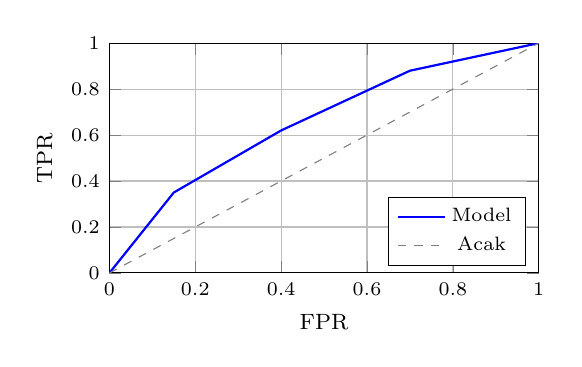
\begin{tikzpicture}
\begin{axis}[
  width=0.58\textwidth,
  height=4.5cm,
  xmin=0, xmax=1,
  ymin=0, ymax=1,
  xlabel={\footnotesize FPR},
  ylabel={\footnotesize TPR},
  grid=major,
  tick label style={font=\scriptsize},
  legend style={font=\scriptsize, at={(0.97,0.03)}, anchor=south east}
]
\addplot[thick, blue] coordinates {(0,0) (0.15,0.35) (0.4,0.62) (0.7,0.88) (1,1)};
\addplot[dashed, gray] coordinates {(0,0) (1,1)};
\legend{Model, Acak}
\end{axis}
\end{tikzpicture}
\caption{Ilustrasi kurva ROC untuk klasifikasi biner: diagonal putus-putus = baseline acak; kurva di atasnya menandakan pemisahan kelas yang lebih baik (AUC lebih besar).}
\end{figure}
